\documentclass[a4paper]{article}

\usepackage{graphicx}
\usepackage{tocloft}
\usepackage{amsmath, amssymb}
\usepackage[top=20mm, bottom=20mm, left=20mm, right=20mm]{geometry}
\usepackage[bookmarks=false,pdfstartview=FitH,colorlinks=false]{hyperref}
\usepackage{fancyhdr}
\usepackage{tikz}
\usepackage{verbatim}
\usepackage{titlesec}
\usepackage{makecell}

\usetikzlibrary{snakes}
\usetikzlibrary{shapes.geometric}
\usetikzlibrary{shapes.misc}

\def\({\left(}
\def\){\right)}
\def\[{\left[}
\def\]{\right]}

\newcommand{\beq}{\begin{equation}}
\newcommand{\eeq}{\end{equation}}
\newcommand{\beqq}{\begin{equation*}}
\newcommand{\eeqq}{\end{equation*}}
\newcommand\beqa{\begin{eqnarray}}
\newcommand\eeqa{\end{eqnarray}}
\newcommand\bea{\begin{array}}
\newcommand\eea{\end{array}}

%\DeclareMathOperator{\tr}{Tr}
\DeclareMathOperator{\str}{STr}

\newcommand{\bra}[1]{\langle #1|}
\newcommand{\ket}[1]{|#1\rangle}
\newcommand{\braket}[2]{\langle #1|#2\rangle}
\newcommand{\tr}{\mathrm{Tr}}
\newcommand{\N}{\mathcal{N}}
\newcommand{\ord}[1]{\mathcal{O}\left(#1\right)}
\newcommand{\adsfive}{AdS_5 \times S^5}
\newcommand{\adscp}{AdS_{4}\times \mathbb{CP}^{3}}
\newcommand{\pmu}{{\bf P}\mu}

\newcommand{\mc}{\mathcal }
\newcommand{\nn}{\nonumber}

\def\bP{{\bf P}}
\newcommand{\mZ}{{\mathbb Z}}
\newcommand{\sh}{{\rm sh}}
\newcommand{\ch}{{\rm ch}}

\newcommand{\M}{{\cal M}}

\newcommand{\pd}{\partial}

\newcommand{\eq}[1]{(\ref{#1})}

\hypersetup{pdfborder = {0 0 0}}

\numberwithin{equation}{section}

\setlength{\cftaftertoctitleskip}{40pt}
\setlength{\cftbeforesubsecskip}{5pt}

\titlespacing*{\section}{0pt}{5.5ex plus 1ex minus .2ex}{4.3ex plus .2ex}
\titlespacing*{\subsection}{0pt}{5.5ex plus 1ex minus .2ex}{4.3ex plus .2ex}

\linespread{1.5}

\begin{document}

\begin{titlepage}

\thispagestyle{empty}

\begin{center}

\begin{figure}[t]
	\centering
	
\includegraphics[width=0.25\textwidth]{../graphics/kcl_logo}
\end{figure}

\vspace*{50pt}

\LARGE
\textbf{Exact Results in Supersymmetric Gauge Theories}

\vspace{40pt}

\Large
Saulius Valatka

\vspace{30pt}

\small
\it{Department of Mathematics, King's College London, \\
Strand, London WC2R 2LS, U.K.}

\vspace{230pt}

\Large\rm
Thesis supervisor Dr. Nikolay Gromov

\vspace{30pt}

\small
Thesis submitted in partial fulfilment of the requirements \\
of the Degree of Doctor of Philosophy

\vspace{40pt}

\large
September 2014

\end{center}

\end{titlepage}


\newgeometry{top=30mm, bottom=25mm, left=40mm, right=25mm}
\pagestyle{fancy}



\section*{Abstract}

\vspace{30pt}

Lorem ipsum dolor sit amet, consectetur adipiscing elit. Fusce at lacus ornare, fringilla velit id, blandit metus. Sed mattis, tortor et rutrum ultrices, elit erat fringilla est, nec semper sem nunc ac ante. Sed placerat sapien eu egestas sollicitudin. Nunc pretium purus justo, non pretium lorem tempus non. Vivamus rhoncus sit amet urna vitae vestibulum. Phasellus dignissim nunc ac felis egestas, nec porta ligula pulvinar. Nulla malesuada sapien nec lobortis dapibus. Morbi auctor nibh felis, at eleifend tellus venenatis et. Sed euismod risus lobortis turpis vulputate, id tincidunt mauris interdum. Quisque sollicitudin bibendum nisl ut feugiat. Cras sed erat fermentum, gravida eros non, placerat felis.

Pellentesque aliquet at risus nec volutpat. In orci enim, ullamcorper ac augue eget, convallis sodales augue. Nulla nec elit pretium, dignissim est nec, tincidunt nisl. Class aptent taciti sociosqu ad litora torquent per conubia nostra, per inceptos himenaeos. In consectetur nec risus eget luctus. Praesent blandit porta tincidunt. In et egestas est. Quisque molestie nulla a dui iaculis, ac placerat neque sollicitudin.

Phasellus ut posuere lectus. Quisque posuere ut nunc sit amet lacinia. Phasellus tempus ut ligula a eleifend. Vestibulum sed ultricies elit, non adipiscing tellus. Vestibulum dignissim velit purus, sit amet pharetra nibh porta quis. Ut et dignissim eros, in condimentum dolor. Etiam sed tempor urna. Proin placerat cursus vestibulum. Aliquam ac dapibus massa. Morbi sit amet sem malesuada, dignissim turpis in, vestibulum ligula. Phasellus vel pharetra lectus, sed molestie orci. Donec placerat consectetur augue non tempus. Proin adipiscing quis purus quis elementum. Nulla facilisi. Vivamus adipiscing diam eu dictum adipiscing.

In sapien orci, viverra in elit iaculis, hendrerit facilisis ipsum. Sed interdum ante ac mattis sollicitudin. Curabitur lacus ligula, fringilla nec arcu eget, venenatis venenatis diam. Nulla eu tellus eget orci cursus convallis. Proin id dui dolor. Praesent eget varius urna, ac condimentum erat. Maecenas interdum mi a varius feugiat. Nunc mi sem, mollis vel quam et, vehicula rhoncus nulla. Cras ac aliquet ipsum, sit amet sagittis ante. In hac habitasse platea dictumst. Vestibulum porta, nulla nec aliquam porta, justo ipsum dignissim lectus, at euismod orci urna quis felis.

Proin id mauris eget diam euismod adipiscing. Nullam imperdiet nunc mollis est rhoncus viverra. Ut rhoncus porttitor tellus sit amet interdum. Donec imperdiet justo risus, in fringilla lectus consectetur id. Quisque tempus tortor neque, eu porta nisi sollicitudin eget. Phasellus hendrerit nisi tellus, quis ullamcorper nunc cursus sed. Integer hendrerit nec dolor in accumsan. Nam vel risus porta, consequat purus sit amet, adipiscing sem. In ultricies erat a facilisis porttitor. Sed varius placerat nunc, vel mollis ante sodales in. Cras egestas arcu in risus gravida scelerisque. Donec quis mattis diam. Proin faucibus euismod dictum. Pellentesque porta molestie laoreet.

\newpage 

%\section*{Acknowledgements}

\vspace{30pt}

First of all I am immensely grateful to Nikolay Gromov for his brilliant supervision and collaboration throughout the years. 
I am also grateful to my colleagues Grigory Sizov and Fedor Levkovich-Maslyuk for all the invaluable discussions and collaborations. In addition I am very thankful to Fedor for thoroughly proofreading this thesis.
The staff and fellow students at King's have all contributed to the three wonderful years I spent there, for that I am very grateful.
I was also lucky enough to travel and visit various institutions around the world where I had the pleasure of meeting fellow scientists, I thank everyone for their hospitality and generosity.
Last but not least I want to thank my family and friends for their support and understanding. 
A special thanks goes to Ieva and Lara, your love and support have helped me stay sane throughout the years.

%\newpage

\tableofcontents

\newpage

% main.tex

\section{Introduction}

The title of this thesis is \emph{Exact Results in $\N=4$ Super Yang-Mills}. A reasonable question to ask is -- why would anyone care about that ? 
After all $\N=4$ is just a toy theory, it is not something that nature implements and thus we can not observe it in particle accelerators, as opposed to say the Standard Model of particle physics. 
And indeed those are all valid points, however there are very good reasons for studying $\N=4$ SYM. 

From a pragmatic point of view, it is the simplest non-trivial quantum field theory in four spacetime dimensions and since attempts at solving realistic QFTs such as the theory of strong interactions (QCD) have so far been futile, it seems like a good starting point -- some go as far as calling it the harmonic oscillator of QFTs. 

Another (and probably the main) reason why $\N=4$ has been receiving so much attention in the last decades is the long list of mysterious and intriguing properties it seems to posses, making it almost an intelectual pursuit of understanding it. 
The theory has been surprising the theoretical physics community from the very beginning: it is a rare instance of a conformal theory in dimensions higher than two, it has a dual description in terms of a string theory and more recently it was discovered to be integrable. 
All of these properties give reasonable hope for actually solving the theory exactly, something that has never been achieved before for any four dimensional interacting QFT.

In the remainder of the section we give a proper introduction to the subject from a historic point of view focusing on its integrability aspect, for it is integrability that allows one to actually find exact results in the theory. We then give an overview of the thesis itself, emphasizing which parts of the text are reviews of known material and which parts constitute original work.

\subsection{Brief history of the subject}

Quantum field theory has been at the spot light of theoretical physics since the beginning of the century when it was found that electromagnetism is described by the theory of quantum electrodynamics (QED). Since then people have been trying to fit other forces of nature into the QFT framework. 
Ultimately it worked: the theory of strong interactions, quantum chromodynamics or QCD for short, together with the electroweak theory, spontaneously broken down to QED, collectively make up the \emph{Standard Model} of particle physics, which has been extensively tested in particle accelerators since then. 

However nature did not give away her secrets without a fight. 
For some time it was though that strong interactions were described by a theory of vibrating strings, as it seemed to incorporate the so-called Regge trajectories observed in experiments \cite{Veneziano:1968}. 
Even after discovering QCD, which is a Yang-Mills gauge theory, stringy aspects of it were still evident and largely mysterious. 
Most notably lattice gauge theory calculations at strong coupling suggested that surfaces of color-electric fluxes between quarks could be given the interpretation of stretched strings \cite{Wilson:1974}, thus an idea of a gauge-string duality was starting to emerge. 
It was strongly re-enforced by t'Hooft, who showed that the perturbative expansion of $U(N)$ gauge theories in the large $N$ limit could be rearranged into a genus expansion of surfaces triangulated by the double-line Feynman graphs, which strongly resembles string theory genus expansions \cite{THooft:1974}.

\vspace{20pt}
\newlength\yearposx
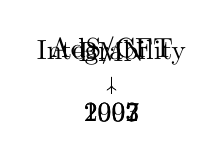
\begin{tikzpicture}[scale=1.6]

    \foreach \x in {1996,1997,2002,2003,2004}{
        \pgfmathsetlength\yearposx{(\x-1996)*1cm};
        \coordinate (y\x)   at (\yearposx,0);
        \coordinate (y\x t) at (\yearposx,+2pt);
        \coordinate (y\x b) at (\yearposx,-2pt);
    }
	
    \draw [->] (y1996) -- (y2004);
    \foreach \x in {1997,2002,2003} \draw (y\x t) -- (y\x b);

	\node at (y1997) [below=3pt] {1997}; \node at (y1997) [above=4pt] {AdS/CFT}; 
	\node at (y2002) [below=3pt] {2002}; \node at (y2002) [above=5pt] {BMN}; 
	\node at (y2003) [below=3pt] {2003}; \node at (y2003) [above=4pt] {Integrability}; 
\end{tikzpicture}
\vspace{20pt}

However it was the work of Maldacena in 1997 that sparked a true revolution \cite{Maldacena:1997re}. 
He formulated the first concrete conjecture, now universally referred to as \emph{AdS/CFT}, for a duality between a gauge theory, the maximally supersymmetric $\N=4$ super Yang-Mills, and type IIB string theory on $\adsfive$. 
Polyakov had already shown that non-critical string theory in four-dimensions describing gauge fields should be complemented with an extra Liouville-like direction thus enriching the space to a curved five dimensional manifold \cite{Polyakov:1997tj}. Furthermore the gauge theory had to be defined on the boundary of this manifold.
Maldacena's conjecture was consistent with this view, as the gauge theory was defined on the boundary of $AdS_5$, whereas the $S^5$ was associated with the internal symmetries of the gauge fields.
The idea of a higher dimensional theory being fully described by a theory living on the boundary was also considered before in the context of black hole physics \cite{'tHooft:1993gx, Susskind:1994vu} and goes by the name of holography.

The duality can be motivated by considering a stack of parallel D3 branes in type IIB string theory. 
Open strings moving on the branes can be described by $\N=4$ SYM with the gauge group $SU(N)$. 
Roughly the idea is that there are six extra dimensions transverse to the stack of branes, thus a string stretching between two of them can be viewed as a set of six scalar fields ${(\Phi^i)^a}_b$ defined in four dimensional spacetime carrying two extra indices denoting the branes it is attached to. 
These are precisely the indices of the adjoint representation of $SU(N)$.
A similar argument can be put forward for other fields thus recovering the field content of $\N=4$ SYM.
Far away from the branes we have closed strings propagating in empty space. 
In the low energy limit these systems decouple and far away from the branes we are left with ten dimensional supergravity.

Another way of looking at this system is considering the branes as a defect in spacetime, which from the point of view of supergravity is a source of curvature. 
The supergravity solution carrying D3 brane charge can be written down explicity \cite{Horowitz:1991cd}.
Far away from the branes it is obviously once again the usual flat space ten dimensional supergravity.
However the near horizon geometry of the brane system becomes $\adsfive$.

Since both points of view end up with supergravity far away from the branes, one is tempted to identify the theories close to the branes -- $\N=4$ SYM and type IIB string theory on $\adsfive$. 
This is exactly what Maldacena did in his seminal paper \cite{Maldacena:1997re}. Since then other dualities have been discovered that are very similar in spirit \cite{Aharony:2008ug}, however in this thesis we will only concentrate on the original one.

By studying the supergravity solution one can identify the parameters of the theories, namely $\N=4$ SYM is parameterized by the coupling constant $g_{YM}$ and the number of colors $N$, whereas string theory has the string coupling constant $g_s$ and the string length squared $\alpha'$. 
These are identified in the following way
\beq
	 4\pi g_s = g_{YM}^2 \equiv \frac{\lambda}{N}, \;\;\;\;\;\;\; \frac{R^4}{\alpha'^2} = \lambda,
\eeq
where $\lambda$ is the t'Hooft coupling and $R$ is the radius of both $AdS_5$ and $S_5$, which is fixed as only the ratio $R^2/\alpha'$ is measurable.
A few things are to be noted here. First of all, the identification directly implements t'Hooft's idea of large $N$ expansion of gauge theory, since $g_s \sim 1/N$. 
In fact in the large $N$ limit only planar Feynman graphs survive and everything simplifies dramatically, a fact that we will take advantage of a lot in this thesis.
In this limit the effective coupling constant of the gauge theory is $\lambda$. 

The supergravity approximation is valid when $\alpha' \ll R^2$, which corresponds to strongly coupled gauge theory, thus the conjecture is of the weak-strong type. 
This fact is a blessing in disguise, since initially it seems very restrictive as one can not easily compare results of the theories. 
However it provides a possibility to access strongly coupled regimes of both theories, which was beyond reach before. 
Prescriptions for matching up observables on both sides of the correspondence were given in \cite{Gubser:1998bc, Witten:1998qj}. 
However because of the weak-strong nature of the duality initial tests were performed only for BPS states, which are protected from quantum corrections.
The first direct match was observed in \cite{Witten:1998qj} where it was shown that the spectrum of half-BPS single trace operators matches the Kaluza-Klein modes of Type IIB supergravity.

The situation changed dramatically in 2002 when Berenstein, Maldacena and Nastase devised a way to go beyond BPS checks \cite{Berenstein:2002jq}. 
The idea was to take an operator in gauge theory with large R-charge $J$ and add some some impurities, effectively making it ``near-BPS''.
The canonical example of such an operator is $\tr(Z^J X^S)$, where $Z$ and $X$ are two complex scalar fields of $\N=4$ SYM, with $X$ being the impurities ($S \ll J$).
Since anomalous dimensions are suppressed like $\lambda/J^2$, perturbative gauge theory calculations are valid even at large $\lambda$, as long as $\lambda' \equiv \lambda / J^2 \ll 1$ and $N$ is large.
It is thus possible to compare gauge theory calculations with string theory results.
From the string theory point of view this limit corresponds to excitations of point-like strings with angular momentum $J$ moving at the speed of light around the great circle of $S^5$. 
The background seen by this string is the so-called pp-wave geometry and string theory in this background is tractible.

The discovery of the BMN limit was arguably the first time it was explicitly demonstrated how the world sheet theory of a string can be reconstructed by a physical picture of scalar fields dubbed as ``impurities'' propagating in a closed single trace operator of ``background'' scalar fields of the gauge theory. 
Shortly after this discovery Minahan and Zarembo revolutionized the subject once again by discovering Integrability at the end of 2002 \cite{Minahan:2002ve}.
They showed that single-trace operators of scalar fields can be identified with spin chains and their anomalous dimensions at one-loop in weak coupling are given by the energies of the corresponding spin chain states.
These spin-chain systems are known to be integrable, which in practice allows one to solve the problem exactly using techniques such as the Bethe ansatz \cite{Bethe:1931}. 
This discovery sparked a very rapid development of integrability methods in AdS/CFT during the coming years.

\vspace{20pt}
\begin{tikzpicture}[scale=3.87]
    
	\coordinate (start) at (0,0);
	\coordinate (end) at (3.3cm,0);
	
    \foreach \x in {2003,2004,2005,2006}{
        \pgfmathsetlength\yearposx{((\x-2003)*1cm + 0.1cm)};
        \coordinate (y\x)   at (\yearposx,0);
        \coordinate (y\x t) at (\yearposx,+0.5pt);
        \coordinate (y\x b) at (\yearposx,-0.5pt);
    }
	
    \draw [->] (start) -- (end);
    \foreach \x in {2003,2004,2005,2006} \draw (y\x t) -- (y\x b);

	\node at (y2003) [below=3pt] {2003}; 
	\node at (y2004) [below=3pt] {2004}; 
		% \node at (y2003) [above=4pt] {AdS/CFT}; 
	\node at (y2005) [below=3pt] {2005}; 
		% \node at (y2004) [above=5pt] {KMMZ}; 
	\node at (y2006) [below=3pt] {2006}; 
		% \node at (y2006) [above=4pt] {ABA}; 
\end{tikzpicture}
\vspace{20pt}

Very rapid development.

\vspace{20pt}
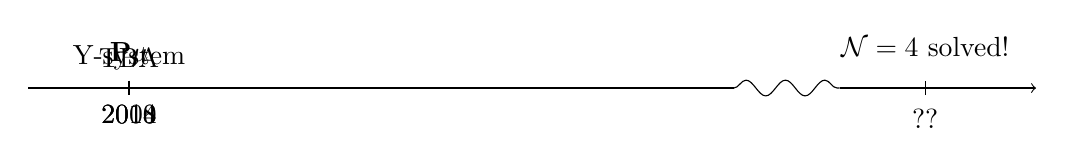
\begin{tikzpicture}[scale=1.28]

	\coordinate (start) at (0,0);
	\coordinate (end) at (6.5cm,0);
	
    \foreach \x in {2008,2009,2010,2012,2014}{
        \pgfmathsetlength\yearposx{(\x-2008)*1cm + 0.4cm};
        \coordinate (y\x)   at (\yearposx,0);
        \coordinate (y\x t) at (\yearposx,+2pt);
        \coordinate (y\x b) at (\yearposx,-2pt);
    }
    
    \draw [-] (0,0) -- (7cm,0);
    \draw [decorate, decoration={snake, segment length=5mm, amplitude=1mm}] (7cm,0) -- (8.05cm,0);
	\draw [->] (8.05cm,0) -- (10cm,0);
	
	\foreach \x in {2008,2010,2014} \draw (y\x t) -- (y\x b);
	
    \node at (y2008) [below=3pt] {2008}; \node at (y2008) [above=4pt] {TBA}; 
	\node at (y2010) [below=3pt] {2010}; \node at (y2010) [above=3pt] {Y-system}; 
	\node at (y2014) [below=3pt] {2014}; \node at (y2014) [above=4pt] {$\pmu$}; 
		
	\draw (8.9cm,-2pt) -- (8.9cm,+2pt);
	\node at (8.9cm,0) [below=4pt] {??}; \node at (8.9cm,0) [above=8pt] {$\N=4$ solved!}; 
	
\end{tikzpicture}
\vspace{20pt}

Exact solutions. Bright future ahead.

\subsection{Thesis overview}

Maybe a nice picture for the structure of the thesis.


\newpage 

% main.tex

\section{$\N=4$ super Yang-Mills}
\label{sec:cft}

\begin{chapquote}{German Proverb}
The devil is in the details.
\end{chapquote}

\noindent For the most part of this thesis we will be dealing with $\N=4$ super Yang-Mills theory. 
In this chapter we start off by defining it via its action and discussing its symmetries and observables. 
We also give an alternative formulation of the theory as a string theory, which is the core idea of the AdS/CFT correspondence. 
This formulation will later prove to be incredibly useful when discussing integrability and exact solutions.

\subsection{Action}

$\N=4$ super Yang-Mills theory is a quantum field theory much like the Standard Model of particle physics with a certain field content and interaction pattern.
It was first discovered by considering $\N=1$ super Yang-Mills theory in $9+1$ spacetime dimensions \cite{Brink:1977}, its action is given by
\begin{equation}
	S = \int d^{10} x \, \mathrm{Tr} \, \left( -\frac{1}{4}  F_{MN} F^{MN}  + \frac{1}{2} \bar{\Psi} \Gamma^M \mathcal{D}_M \Psi \right), \; \quad \; M = 1 \dots 10,
\end{equation}
where $\Psi$ is a Majorana-Weyl spinor in $9+1$ dimensions with $16$ real components and $\Gamma^M$ are the appropriate gamma matrices. 
The covariant derivative $\mathcal{D}_M$ is defined as
\begin{equation}
	\mathcal{D}_M = \partial_M - ig_{YM} \; [A_M, \, ],
\end{equation}
where $g_{YM}$ is the Yang-Mills coupling constant. 
The gauge group is in principle arbitrary, but we choose $SU(N)$ in anticipation of the AdS/CFT correspondence. 
By dimensionally reducing this theory on a flat torus $T^6$ one recovers the maximally supersymmetric $\N=4$ Yang-Mills gauge theory in $3+1$ spacetime dimensions.
The reduced action reads
\begin{equation}
\begin{split}
S = & \int d^4 x \, \tr \, \left( -\frac{1}{2} \mathcal{D}_\mu \Phi_I \mathcal{D}^\mu \Phi^I  + \frac{g_{YM}^2}{4} [\Phi_I, \Phi_J] [\Phi^I, \Phi^J] - \frac{1}{4}  F_{\mu\nu} F^{\mu\nu}  \right. \\
	 &\left. - \bar{\psi}^a \sigma^\mu \mathcal{D}_\mu \psi_a  + \frac{ig_{YM}}{2} \sigma^{ab}_I \psi_a [\Phi^I, \psi_b] + \frac{ig_{YM}}{2} \sigma_{ab}^I \bar{\psi}^a [\Phi_I, \bar{\psi}^b] \right).
\end{split}
\label{eq:n4_action}
\end{equation}
After dimensional reduction the gauge field $A_M$ decomposes to the four dimensional gauge field $A_\mu$ and to six real scalar fields $\Phi_I$ whereas the Majorana-Weyl spinor $\Psi_A$ breaks up into four copies of the left and right Weyl spinors in four dimensions 
\begin{equation}
	\Psi_A \, \, (A = 1, ..., 16) \, \, \, \rightarrow \, \, \,  \bar{\psi}^a_{\dot{\alpha}}, \; \psi_{a\alpha} \, \, (\alpha, \dot{\alpha} = 1, 2, \; \; a = 1, ..., 4).
\end{equation}
It also gives rise to the $SO(6) \simeq SU(4)$ symmetry called \emph{R-symmetry}, which originally was part of the ten dimensional Poincare group, but now acts as an internal symmetry of the supercharges.
It permutes the scalars, which live in the fundamental ${\bf 6}$ of $SO(6)$ and the spinors, which live in the fundamental of $SU(4)$, namely the lower index $a$ in $\psi_{a\alpha}$ transforms in ${\bf 4}$, while $\bar{\psi}_{\dot{\alpha}}^a$ transforms in ${\bf \bar{4}}$. 
From this it follows that we can combine the six real scalars $\Phi^I$ into three complex scalars $\Phi^{ab}$, often denoted as $X$, $Y$ and $Z$, which then transform under the second rank antisymmetric ${\bf 6}$ of $SU(4)$. 
The gauge field is a singlet under R-symmetry.

It is now a straightforward but rather tedious task to calculate the beta function for this theory. 
For any $SU(N)$ gauge theory at one loop level it is given by \cite{Gross:1973}
\begin{equation}
	\beta(g) = - \frac{g_{YM}^3}{16\pi^2} \left( \frac{11}{3} N - \frac{1}{6} \sum_s C_s - \frac{1}{3} \sum_f \tilde{C}_f \right)
\end{equation}
where the first sum is over the real scalars and the second one over the fermions. 
$C_s$ and $\tilde{C}_f$ are the quadratic Casimirs, which in our case are equal to $N$ since all fields are in the adjoint representation of the group. 
It is then easy to see that at least at one loop level the theory is conformally invariant. 
In fact the $\beta$ function was shown to be identically zero to all orders in perturbation theory \cite{Sohnius:1981ab,Mandelstam:1983, Brink:1983}, hence $\N=4$ super Yang-Mills is fully conformally invariant even after quantization. 
After discussing the full symmetry algebra of the theory and its representations we will give an elegant argument why this is true.

\subsection{Observables}

The theory has 16 on-shell degrees of freedom which make up the gauge multiplet of $\N=4$ supersymmetry, namely $(\Phi_I, \psi_a, A_\mu)$. 
Gauge invariant operators are then formed by taking traces over the gauge group. 
An important class of operators are the \emph{local operators}, which are traces of fields all evaluated at the same spacetime point. 
They have the general form
\begin{eqnarray}
	\mathcal{O}_{i_1 \mu i_2 \alpha \dots i_n \dots j_1 \nu \beta \dots j_n}(x) & = \tr \left[ \Phi_{i_1}(x) \mathcal{D}_\mu \Phi_{i_2}(x) \psi_\alpha(x) \dots \Phi_{i_n}(x) \right] \times \dots \nonumber \\
	& \dots \times \tr \left[ \Phi_{j_1}(x) \mathcal{D}_\nu \psi_\beta(x) \dots \Phi_{j_n}(x) \right]. 
\end{eqnarray} 
In this thesis we will be exclusively focusing on the planar limit, which is the limit when the number of colors $N$ is sent to infinity. 
Diagrams involving multi-trace operators are non-planar, hence suppressed in the large $N$ limit and therefore we will only be considering single trace operators.
An example of a non-local operator is the Wilson loop, given by
\beq
	W_L= \tr \, \( {\mathcal P}\exp\!\oint_C \! dt\(i  A\cdot\dot{x}+\vec\Phi\cdot\vec n\,|\dot x|\) \),
\eeq
which depends on the path $x^\mu(t)$ in spacetime, hence it is known as a \emph{line operator}. 
It also depends on the coupling to the scalar fields, which is encoded in the six-dimensional unit vector $\vec{n}(t)$. 
The scalar field term can also be understood by recalling that the scalar fields are a result of dimensional reduction from $9+1$ dimensions, thus the coupling vector $\vec{n}(t)$ together with the curve $x^\mu(t)$ make up a path $x^M(t)$ in $9+1$ dimensional spacetime. 
In later sections of the text we will be considering cusped Wilson lines with other operators inserted at the cusp. We will be mostly working in these two classes of operators, however in principle one could go on and define surface operators, etc.

\subsection{Symmetry}

Conformal symmetry, supersymmetry and R-symmetry are a part of a bigger group $PSU(2,2|4)$, which is also known as the \emph{$\N=4$ superconformal group}. 
It is the full symmetry group of $\N=4$ super Yang-Mills and is unbroken by quantum corrections. 
It is an example of a \emph{supergroup}, i.e. a graded group containing bosonic and fermionic generators. 
The theory of supergroups is highly developed \cite{Sohnius:1981ab,Mandelstam:1983, Brink:1983,Beisert:2010kp} and much of the techniques from studying bosonic groups carry over to supergroups with some additional complications, i.e. Dynkin diagrams, root spaces, weights etc. 

$PSU(2,2|4)$ has the bosonic subgroup of $SU(2,2) \times SU(4)$, where $SU(2,2) \simeq SO(2,4)$ is the conformal group in four dimensions and $SU(4) \simeq SO(6)$ is the R-symmetry. 
The conformal group has the Poincar\'{e} group as a subgroup, which has a total of 10 generators including four translations $P_\mu$ and six Lorentz transformations $M_{\mu\nu}$, in addition there is the generator for dilatations $D$ and four special conformal generators $K_\mu$. 
Their commutation relations read
\begin{eqnarray}
 &[D, M_{\mu\nu}] = 0 \; \; \; [D, P_\mu] = -i P_\mu \; \; \; [D, K_\mu] = +i K_\mu,  \nonumber\\
 &[M_{\mu\nu}, P_\lambda] = -i(\eta_{\mu\nu} P_\nu - \eta_{\lambda\nu} P_\mu) \; \; \; [M_{\mu\nu}, K_\lambda] = -i(\eta_{\mu\lambda} K_\nu - \eta_{\lambda\nu} K_\mu),  \nonumber\\
 &[P_\mu, K_\nu] = 2i(M_{\mu\nu} - \eta_{\mu\nu} D).
 \label{eq:conformal_group}
\end{eqnarray}
$\N=4$ supersymmetry has 16 supercharges $Q_{a\alpha}$ and $\tilde{Q}^a_{\dot{\alpha}}$ where $\alpha, \dot{\alpha} = 1, 2$ are the Weyl spinor indices and $a = 1,...,4$ are the R-symmetry indices. 
These generators have the usual commutation and anti-commutation relations with the Poincar\'{e} generators given by 
\begin{eqnarray}
	& \{Q_{\alpha a}, \tilde{Q}^b_{\dot{\alpha}}\} = \gamma^\mu_{\alpha\dot{\alpha}} \delta_a^b P_\mu \; \; \; \{Q_{\alpha a}, Q_{\alpha b}\} = \{ \tilde{Q}^a_{\dot{\alpha}}, \tilde{Q}^b_{\dot{\alpha}} \} = 0, \nonumber\\
	& [M^{\mu\nu}, Q_{\alpha a}] = i \gamma^{\mu\nu}_{\alpha\beta} \epsilon^{\beta\gamma} Q_{\gamma a} \; \; \; [M^{\mu\nu}, \tilde{Q}^a_{\dot{\alpha}}] = i \gamma^{\mu\nu}_{\dot{\alpha}\dot{\beta}} \epsilon^{\dot{\beta}\dot{\gamma}} \tilde{Q}_{\dot{\gamma}}^a, \nonumber \\
	& [P_\mu, Q_{\alpha a}] = [P_\mu, \tilde{Q}^b_{\dot{\alpha}}] = 0,
\end{eqnarray} 
where $\gamma_{\alpha\beta}^{\mu\nu} = \gamma^{[\mu}_{\alpha\dot{\alpha}} \gamma^{\nu]}_{\beta\dot{\beta}} \epsilon^{\dot{\alpha}\dot{\beta}}$. 
Commutators between supercharges and the conformal generators are also non trivial and introduce new supercharges,
\begin{eqnarray}
	& [D, Q_{\alpha a}] = -\frac{i}{2} Q_{\alpha a} \; \; \; [D, \tilde{Q}_{\dot{\alpha}}^a] = -\frac{i}{2} \tilde{Q}_{\dot{\alpha}}^a, \nonumber \\
	& [K^\mu,  Q_{\alpha a}] = \gamma^\mu_{\alpha\dot{\alpha}} \epsilon^{\dot{\alpha} \dot{\beta}} \tilde{S}_{\dot{\beta} a} \; \; \; [K^\mu, \tilde{Q}_{\dot{\alpha}}^a] = \gamma^\mu_{\alpha\dot{\alpha}} \epsilon^{\alpha\beta} S_\beta^a,
	\label{eq:dq_commutators}
\end{eqnarray}
where $\tilde{S}_{\dot{\alpha} a}$ and $S_\alpha^a$ are the \emph{special conformal supercharges}. 
They have opposite \text{R-symmetry} representations compared to the usual supercharges. 
The special supercharges bring the total of supercharges to 32. 
The commutation and anti-commutation relations for the special conformal supercharges are very much like the ones for normal supercharges,
\begin{eqnarray}
	& \{S_{\alpha}^a, \tilde{S}_{\dot{\alpha} b}\} = \gamma^\mu_{\alpha\dot{\alpha}} \delta_b^a K_\mu \; \; \; \{S_{\alpha}^a, S_{\alpha}^b\} = \{ \tilde{S}_{\dot{\alpha} a}, \tilde{S}_{\dot{\alpha} b} \} = 0, \nonumber\\
	& [M^{\mu\nu}, S_{\alpha}^a] = i \gamma^{\mu\nu}_{\alpha\beta} \epsilon^{\beta\gamma} S_{\gamma}^a \; \; \; [M^{\mu\nu}, \tilde{S}_{\dot{\alpha} a}] = i \gamma^{\mu\nu}_{\dot{\alpha}\dot{\beta}} \epsilon^{\dot{\beta}\dot{\gamma}} \tilde{S}_{\dot{\gamma} a}, \nonumber \\
	& [K_\mu, S_{\alpha}^a] = [K_\mu, \tilde{S}_{\dot{\alpha} a}] = 0.
\end{eqnarray} 
Finally the anti-commutation relations between the special conformal and usual supercharges close the algebra,
\begin{eqnarray}
	\{ Q_{\alpha a}, S_\beta^b \} & = & - i \epsilon_{\alpha\beta} {{\sigma^{IJ}}_a}^b R_{IJ} + \gamma_{\alpha\beta}^{\mu\nu} {\delta_a}^b M_{\mu\nu} - \frac{1}{2} \epsilon_{\alpha\beta} {\delta_a}^b D \nonumber \\
	\{ \tilde{Q}_{\dot{\alpha}}^a, \tilde{S}_{\dot{\beta} b} \} & = & + i \epsilon_{\dot{\alpha}\dot{\beta}} {{\sigma^{IJ}}^a}_b R_{IJ} + \gamma_{\dot{\alpha}\dot{\beta}}^{\mu\nu} {\delta^a}_b M_{\mu\nu} - \frac{1}{2} \epsilon_{\dot{\alpha}\dot{\beta}} {\delta^a}_b D \nonumber \\
	\{ Q_{\alpha a}, \tilde{S}_{\dot{\beta} b} \} & = & \{ \tilde{Q}_{\dot{\alpha}}^a, S_\beta^b \} = 0
	\label{eq:qs_anticommutators}
\end{eqnarray}
where $R_{IJ}$ are the generators of R-symmetry with $I,J = 1, ..., 6$. 
All supercharges transform under the two spinor representations of the R-symmetry group and all other generators commute with it. 
All of the generators can be organized as follows
\beq
\(
	\begin{array}{c|c}
	K^\mu, P^\mu, M^{\mu\nu}, D & Q_{a\alpha}, \bar{S}_{a\dot{\alpha}} \\ \hline 
	S_{\alpha}^a, \bar{Q}_{\dot{\alpha}}^a  & R_{IJ}
	\end{array} 
\)
\eeq
where the generators in the diagonal blocks are bosonic and the ones in the anti-diagonal blocks are fermionic.
They have a definite dimensions, which are not modified by radiative corrections
\beq
	[D]=[R]=0\;, \quad [P]=1\;, \ [K]=-1\;, \quad [Q]=1/2\;,\  [S]=-1/2\;.
\eeq
In contrast, the classical dimensions of fields
\beq
	[\Phi^I] = [A_\mu] = 1\;, \quad [\psi_a] = \frac{3}{2},
\eeq
do receive radiative corrections and acquire \emph{anomalous dimensions}, which together with the bare dimension make up the conformal dimension
\beq
	\Delta = \Delta_0 + \gamma(g_{YM}).
\eeq
The name is justified by the fact that in conformal field theories all two point functions are determined by the scaling dimensions of the fields. 
More than that, together with the knowledge of all three point functions they are enough to determine any $n$-point function. 
This is why finding conformal dimensions of all operators, i.e. the spectrum of the theory is a very important step in solving it.

\subsubsection{Superconformal multiplets}

Fields of the theory can be organized in unitary representations of the superconformal symmetry group, which are labeled by quantum numbers of the bosonic subgroup
\beqa
	&SO(1,3) \times SO(1,1) \times SU(4) \nonumber \\
	&\quad \; (s_+, s_-) \quad \quad \Delta \quad \quad  [r_1, r_2, r_3]
\eeqa 
where $(s_+, s_-)$ are the usual positive half-integer spin labels of the Lorentz group, $\Delta$ is the positive conformal dimension that can depend on the coupling and $[r_1, r_2, r_3]$ are Dynkin labels of the $R$-symmetry.
All unitary representations of the superconformal group have been classified into four families \cite{Dobrev:1985ab,Dobrev:1985cd}, here we give a short description of the classification.
  
Looking at the commutation relations of the conformal subgroup (\ref{eq:conformal_group}), we see that the operators $P_\mu$ and $K_\mu$ act as raising and lowering operators for the dilatation operator $D$ -- this gives a hint as to how we could construct representations of the group. 
The dilatation operator $D$ is the generator of scalings, i.e. upon a rescaling $x \rightarrow \lambda x$ a local operator in a field theory scales as 
\begin{equation}
	\mathcal{O}(x) \rightarrow \lambda^{-\Delta} \mathcal{O}(\lambda x)
\end{equation}
where $\Delta$ is the conformal dimension of the operator $\mathcal{O}(x)$. 
Restricting to the point $x = 0$, which is a fixed point of scalings, we see that the conformal dimension is the eigenvalue of the dilatation operator,
\begin{equation}
	[D,\mathcal{O}(0)] = -i \Delta \mathcal{O}(0).
\end{equation}
It is now clear that acting on a field with $K_\mu$ should lower the dimension by one and acting with $P_\mu$ -- raise it by one. 
We can show this explicitly using the Jacobi identity as
\beq
	[D, [K_\mu, \mathcal{O}(0)]] = [[D, K_\mu], \mathcal{O}(0)] + [K_\mu, [D, \mathcal{O}(0)]] = -i (\Delta - 1) \; [K_\mu, \mathcal{O}(0)].
\eeq
Since operators in a unitary quantum field theory should have positive dimensions (aside from the identity operator), we should not be able to keep lowering the dimension indefinitely, i.e. there should always be an operator that satisfies
\begin{equation}
	[K_\mu, \tilde{\mathcal{O}}(0)] = 0.
\end{equation} 
We call such operators \emph{conformal primary operators}. 
Acting on these with $P_\mu$ keeps producing operators with a dimension one higher -- we call these the \emph{descendants} of $\tilde{\mathcal{O}}(0)$. 
We can also act with the supercharges and looking at the commutators in (\ref{eq:dq_commutators}) we see that they raise the dimension by $1/2$, while the special conformal supercharges lower it by $1/2$. 
Operators annihilated by special conformal supercharges are called \emph{superconformal primaries}, which is a stronger condition that being a conformal primary.

(Super-)conformal primaries and their descendants make up multiplets that constitute the three families of discrete representations in the classification.
They are further distinguished by the number of supercharges the primary commutes with.
One example is a class of operators that satisfy the condition 
\beq
	\label{eq:halfBPS}
	\Delta = r_1 + r_2 + r_3,
\eeq 
a canonical representative would be a single-trace symmetrized scalar field operator such as 
\beq
	\mathcal{O}^{i j \dots k}(x) = \tr \( \Phi(x)^{(i} \Phi(x)^j \dots \Phi(x)^{k)} \).
\eeq
These operators commute with half of the supercharges, thus they are referred to as \text{half-BPS}. 
A key fact is that operators in the same representation must have the same anomalous dimension, because the generators of the group can only change it by half integer steps and there's only a finite number of generators. 
What is more, operators in the discrete BPS representations are protected from quantum corrections, because at any coupling the total dimension is always algebraically related to the Dynkin labels of the R-symmetry, e.g. as in \eq{eq:halfBPS}. 
Since charges of compact groups are quantized it must mean that the dimension can't continuously depend on the coupling and hence the anomalous dimension must vanish. 
This is however not true for the fourth continuous non-BPS family of representations, hence operators from these multiplets do acquire anomalous dimensions.

Let us conclude the section with an elegant argument for why the beta function of $\N=4$ super Yang-Mills is zero.
One can use the algebra and shown that the operators $\tr \, F_+ F_+$ and $\tr \, F_- F_- $, where $F_\mp$ are the (anti-)self-dual field strengths, belong to the same multiplet as a superconformal primary \cite{Minahan:2010js}, meaning that the $\tr \, F_{\mu\nu} F^{\mu\nu}$ term in the Lagrangian is protected from quantum corrections, hence so is the coupling constant $g_{YM}$. 
This argument is valid to all orders in perturbation theory, which means that $\N=4$ super Yang-Mills is conformally invariant to all orders in perturbation theory.

\subsection{String description at strong coupling}
\label{sec:n4_strong}

As already briefly explained in the introduction, the AdS/CFT conjecture states that $\N=4$ super Yang-Mills is exactly dual to type IIB string theory on $\adsfive$, \cite{Maldacena:1997re,Gubser:1998bc,Witten:1998qj}. 
To be more precise, the gauge group of the Yang-Mills theory is taken to be $SU(N)$ and the coupling constant $g_{YM}$. 
The string theory is defined on $\adsfive$ where both $AdS_5$ and $S^5$ have radius $R$. 
The self-dual five-form field $F_5^+$ has integer flux through the sphere
\beq
	\int_{S^5} F_5^+ = N,
\eeq
and $N$ is identified with the number of colours in the gauge theory. 
The string theory is further parametrized by the string coupling $g_s$ and the string length squared $\alpha'$. The following relations are conjectured to hold
\beq
	 4\pi g_s = g_{YM}^2 \equiv \frac{\lambda}{N}, \;\;\;\;\;\;\; \frac{R^4}{\alpha'^2} = \lambda,
\eeq
where $\lambda$ is the t'Hooft coupling. We will be working in the planar limit $N \rightarrow \infty$ with $\lambda$ fixed. 
It is easy to see that in this limit $g_s \rightarrow 0$ and we are left with freely propagating strings.
Furthermore, the regime of strongly coupled gauge theory when $\lambda \rightarrow \infty$ corresponds to the regime of string theory where the supegravity approximation is valid, namely $\alpha' \ll R^2$.
The takeaway here is that one can formulate strongly coupled planar $\N=4$ super Yang-Mills as a classical theory of free strings on $\adsfive$.


\subsubsection{Sigma model formulation}

A very useful formulation of string theory on $AdS_5 \times S^5$ is the coset space sigma model \cite{Metsaev:1998it} with the target superspace of
\begin{equation}
	\frac{PSU(2,2|4)}{SO(1,4) \times SO(5)}.
\end{equation}
\vspace{2pt}
The bosonic part of the supercoset where the string moves is given by
\beq
	\frac{SO(2,4) \times SO(6)}{SO(1,4) \times SO(5)} = \adsfive,
\eeq
which is constructed as the coset between the isometry and isotropy groups of $\adsfive$. 
The action is then written in terms of the algebra of $PSU(2,2|4)$.

The superalgebra $\alg{psu}{2,2|4}$ has no realization in terms of matrices, instead it is the quotient of $\alg{su}{2,2|4}$ by matrices proportional to the identity. 
On the other hand $\alg{su}{2,2|4}$ is a matrix superalgebra spanned by $8\times8$ supertraceless matrices
\beq
M = \( {\begin{array}{c|c}
 A & B  \\
 \hline
 C & D  \\
 \end{array} } \),
\eeq
where the supertrace is defined as 
\beq
\str M = \tr A - \tr D.
\eeq
$A$ and $D$ are elements of $\alg{su}{2,2}$ and $\alg{su}{4}$ respectively, whereas the fermionic components are related by
\beq
	C = \( {\begin{array}{c|c}
 +\mathbbm{1}_{2\times2} & 0  \\
 \hline
 0 & -\mathbbm{1}_{2\times2}  \\
 \end{array} } \) B^\dagger.
\eeq
An important feature of this algebra is the following automorphism
\beq
\Omega \circ M = \( {\begin{array}{c|c}
 E A^T E & -E C^T E  \\
 \hline
 E B^T E & E D^T E \\
 \end{array} } \),
 \; \quad  \;
E = \( {\begin{array}{cccc}
 0 & -1 & 0 & 0  \\
 1 & 0 & 0 & 0 \\
 0 & 0 & 0 & -1  \\
 0 & 0 & 1 & 0 \\
 \end{array} } \),
\eeq
which endows the algebra with a $\mathbb{Z}_4$ grading, since one can easily check that $\Omega^4 = 1$.
This in turn means that any element of the algebra can be decomposed under this grading as
\beq
	M = \sum_{i=0}^3 M^{(i)},
\eeq
where
\beqa
	\label{eq:M_components}
	M^{(0,2)} &= \frac{1}{2} \( {\begin{array}{c|c}
 A \;\, \pm E A^T E & 0  \\
 \hline
 0 & D \pm E D^T E  \nonumber \\
 \end{array} } \) \\
 M^{(1,3)} &= \frac{1}{2} \( {\begin{array}{c|c}
 0 & B \pm i E C^T E  \\
 \hline
 C \mp i E B^T E & 0  \\
 \end{array} } \)
\eeqa 
and the morphism then acts on the elements of the decomposition as
\beq
	\Omega \circ M^{(n)} = i^n M^{(n)}.
\eeq
The Metsaev-Tseytlin action for the Green-Schwarz superstring is then given by
\begin{equation}
	\label{eq:mt_action}
	S = \frac{\sqrt{\lambda}}{4 \pi} \int \str \left( J^{(2)} \wedge * J^{(2)} - J^{(1)} \wedge J^{(3)} + \Lambda \wedge J^{(2)} \right),
\end{equation}
which is written down in terms of the graded elements of the algebra current
\begin{equation}
	J = -g^{-1} \mathrm{d} g %\in \mathfrak{psu(2,2|4)},
	\label{eq:j_current}
\end{equation}
where $g(\sigma, \tau) \in PSU(2,2|4)$ is a map from the string worldsheet to the supergroup $PSU(2,2|4)$. 
The last term contains a Lagrange multiplier $\Lambda$, which ensures that $J^{(2)}$ is supertraceless, whereas all other components are manifestly traceless as seen from \eq{eq:M_components}. 
Since the target space is the coset of $PSU(2,2|4)$ by $SO(1,4) \times SO(5)$, the map $g$ has an extra gauge symmetry
\begin{equation}
	g \rightarrow gH, \,\,\,\,\, H \in SO(1,4) \times SO(5)
\end{equation}
under which the components of the supercurrent transform as
\beqa
	& J^{(0)} \rightarrow H^{-1} J^{(0)} H - H^{-1} \mathrm{d} H \\
	& J^{(i)} \rightarrow H^{-1} J^{(i)} H, \quad i=1,2,3
\eeqa
The equations of motion read
\beq
	d * k = 0,
\eeq
where $k = gKg^{-1}$ and
\beq
	K = J^{(2)} + \frac{1}{2} * J^{(1)} - \frac{1}{2} * J^{(3)} - \frac{1}{2} * \Lambda.
\eeq
They are equivalent to the conservation of the Noether current associated to the global left $PSU(2,2|4)$ multiplication symmetry.

Finally let us briefly remark on how the action reduces to the usual sigma model action if one restricts to bosonic fields. 
A purely bosonic representative of $PSU(2,2|4)$ has the form
\beq
	g = \( {\begin{array}{c|c}
 A & 0  \\
 \hline
 0 & D  \\
 \end{array} } \),
\eeq
where $A \in SO(6) \simeq SU(4)$ and $D \in SO(2,4) \simeq SU(2,2)$. Then we see that $A E A^T$ is a good parametrization of 
\beq
	\frac{SO(6)}{SO(5)} \simeq \frac{SU(4)}{SP(4)} = S^5,
\eeq
since it is invariant under $A \rightarrow A H$ with $H \in SP(4)$. 
Similarly $D E D^T$ parametrizes $AdS_5$. 
If we now define the coordinates $u^i$ and $v^i$ in the following way
\beq
	u^i \Gamma^S_i = A E A^T, \quad \quad v^i \Gamma^A_i = D E D^T,
\eeq
with $\Gamma^S$ and $\Gamma^A$ being the gamma matrices of $SO(6)$ and $SO(2,4)$ respectively, then by construction they will satisfy the following constraints
\beqa
	1 &= u \cdot u \equiv +u_1^2 + u_2^2 + u_3^2 + u_4^2 + u_5^2 + u_6^2 \nonumber \\
	1 &= v \cdot v \equiv -v_1^2 - v_2^2 - v_3^2 - v_4^2 + v_5^2 + v_6^2,
\eeqa
and the action \eq{eq:mt_action} will read
\beq
	S_b = \frac{\sqrt{\lambda}}{4\pi} \int_0^{2\pi} d\sigma \int d\tau \; \sqrt{h} \( h^{\mu\nu} \pd_\mu u \cdot \pd_\nu u + \lambda_u \( u \cdot u - 1 \) - \( u \rightarrow v \) \),
\eeq
which is just the usual non-linear sigma model for a string moving in $\adsfive$.


%\newpage 

%% main.tex 

\section{String description: AdS/CFT}

Here we talk about the alternative description of the theory as strings moving in AdS.

\subsection{Motivation}

Planar diagrams are string interactions.

\subsection{String theory and the duality}

Give details of the string theory, what are the parameters on both sides, how they match up. What are the limits. Anomalous dimensions match string state energies.

\subsection{First tests: BMN, GKP, FT}

Describe these limits, give first eveidence for the duality. Is this where one finds the first strong coupling coefficient to Konishi ?


\newpage 

% main.tex

\section{Perturbative Integrability}

In this section we dive into the magical world of integrability.
Give picture summarizing all techniques and their ranges of applicability.

\subsection{One loop at weak coupling}

Roughly rederive the Minahan/Zarembo result.

\subsubsection{Closed sectors}

talk about closed sectors.

\subsubsection{The $\mathfrak{sl}(2)$ sector}

Give the sl(2) Hamiltonian, example states and energies.

\subsection{Higher loops}

Short example of a two loop Hamiltonian, perturbative corrections for the states found above with contact terms.

\subsection{Asymptotic solution}

Generalize su(2) BAE to all loops, maybe give a simple example. 

\subsubsection{A glimpse ahead: the slope function}

Derive slope from ABA.

\subsection{Strong coupling and the algebraic curve construction}

Describe flat connections, monodromies, sheets etc.

\subsubsection{Folded string}

Give solution

\subsection{String quantization and semi-classics}

Describe the quantization procedure. Derive next coefficient for Konishi.

\subsection{Short strings}

Combine with slope, derive next coeffient for Konishi.

\subsection{Towards the full solution}

Mention nested BAE, full psu(2,2|4) spin chain without going into much detail.


\newpage 

% main.tex

\section{Exact results}

Exact results are rare and important.

\subsection{Solution to the spectral problem}

\subsubsection{TBA and the Y-system}

\subsubsection{The $\pmu$ system}

\subsection{Folded string}

Mention Frolov numerics. Volin's 8(9) ? loops with $\pmu$.

\subsection{Cusped Wilson line}

Bremstahlung result from $\pmu$.

\subsubsection{Classical limit}

Find the curve, matrix models.

\subsection{Revisiting the slope function}

Derive slope from $\pmu$.

\subsection{The curvature function}

Derive curvature from $\pmu$.

\subsubsection{Weak coupling expansion}

Mention weak coupling and how it matches ABA.

\subsubsection{Strong coupling expansion}

Mention strong coupling, be amazed how it matches string theory.

\subsection{Update on short strings}

Combine semiclassics with curvature and finally derive three-loop Konishi coefficient.


\newpage 

% main.tex

\section{ABJM}

\subsection{Definitions}

\subsection{Weak coupling}

\subsection{Algebraic curve}

\subsection{The $\pmu$ system}

\subsubsection{Applications}

\newpage

% main.tex

\section{Conclusions}

In this thesis we addressed exact results in supersymmetric gauge theories, more explicitly results valid at arbitrary values of the coupling constant in the planar limit.
The magic ingredients that helped us do all of this were the AdS/CFT dualities and their integrability.
Let us now summarize the structures we uncovered while exploring these theories and the results they helped us find.

For the major part of the thesis we considered $\N=4$ super Yang-Mills, which is a canonical example of a supersymmetric gauge theory with the ingredients listed above.
First of all it is dual to type IIB strings on $\adsfive$, which is an immensely powerful statement in its own right.
Furthermore both of these theories are integrable, which technically means that one can find as much conserved charges of motion as there are degrees of freedom.
We uncovered integrability on the gauge theory at weak coupling first when in section \ref{sec:integrability_weak} we mapped local gauge invariant operators to long ranged spin chains and the anomalous dimensions of the operators to the energies of the spin chain states.
Remarkably the abstract problem of finding the spectrum of local operators in a conformal field theory is equivalent to finding the spectrum of a very physical spin chain system.
It was at weak coupling where we also found the first exact result, the leading order small spin expansion coefficient of the generalized Konishi anomalous dimension, also known as the slope function. 
Of course it is a lucky discovery because the slope function is not sensitive to finite size effects, which are the major problem plaguing the spin chain picture.
They manifest as spin chain interactions that wrap around the chain.

At strong coupling $\N=4$ super Yang-Mills is more naturally described by type IIB strings on an $\adsfive$ background via the AdS/CFT correspondence. 
We uncovered integrability in this regime as well in section \ref{sec:integrability_strong}.
Here we found a picture of classical spectral curves, which are Riemann surfaces with sheets connected by branch cuts. 
String solutions were then described by quasi-momenta defined on these surfaces and the physical intuition was that each cut corresponded to an excitation of the string, where the sheets connected denoted the polarization, the size of the cut -- the amplitude and the discontinuity going through the branch cut -- the mode number of the excitation.
Amazingly the highly non-trivial motion of strings on a curved background somehow reduced to a description similar to that of a collection of harmonic oscillators.

The highlight of the whole integrability programme is of course the finite coupling regime where the two seemingly different descriptions meet, obviously they have to somehow emerge as limiting cases of some ultimate underlying structure.
In section \ref{sec:pmu_system} we argued that this hidden construction is the quantum algebraic curve. 
By now there are many ways of seeing its emergence from various limits, yet probably the most intuitive explanation is that the classical spectral curve is a type of WKB approximation of the quantum spectral curve, namely the classical quasi-momentum has to be replaced by its quantum version and the analyticity structure of the construction modified.
In a very rough sense the collection of classical harmonic oscillators gets quantized and the quantum quasi-momenta $\bP_a$ can be though of as the wave functions. 

The quantum spectral curve allowed us to rather easily derive the slope function and extend the calculation by finding the next coefficient in the small spin expansion, which we called the curvature function.
Contrary to the slope, the curvature function is sensitive to finite size effects and we indeed found evidence that our result successfully incorporates all of them.
We then used these exact results to find the first three coefficients in the strong coupling expansion of the Konishi anomalous dimension.
We matched them perfectly with available exact numeric data.
Another observable we discussed was the cusped Wilson line, whose expectation value contains the ubiquitous quantity often called the cusp anomalous dimension.
We showed how easily it can be found in the near BPS limit using the quantum spectral curve, even though technically the observable is non-local and the applicability of the construction is naively questionable.
Our exploration of the classical limit at strong coupling and the corresponding dual open string solution provided further evidence that this class of operators is not that different from local operators, as the result was basically a classical spectral curve.

Finally we touched up the ABJM theory which is another famous integrable supersymmetric gauge theory with a string dual.
The quantum spectral curve is also available in this setting and we briefly mentioned a very powerful exact result found with its help, the so-called interpolating function $h(\lambda)$, which basically encodes the relationship between the integrability coupling constant $h$ and the gauge theory coupling constant $\lambda$.
Amazingly this calculation even shed light on possible generalizations of the quantum spectral curve beyond the planar limit.
Roughly speaking the branch cuts of the quantum spectral curve here emerged as condensations of eigenvalues in the complex plane of an $N \times N$ sized matrix.
One can thus cautiously suspect that maybe going beyond the planar limit simply amounts to discretizing the branch cuts of the quantum spectral curve, a second quantization of sorts. 
Obviously at the moment these are just wild speculations.

In conclusion, AdS/CFT dualities and integrability are immensely powerful tools when dealing with gauge theories, so powerful that they enable one to find results exact in the coupling constant.
Obviously the ultimate goal of this research programme is to learn something that could be applied to real world theories such as QCD.
If we knew as much about QCD as we do about $\N=4$ super Yang-Mills by now we could analytically find the mass of the proton.
Unfortunately we are not there yet, but one can dream.






\newpage

\bibliography{bibliography}



\begin{thebibliography} {9}

%\cite{Veneziano:1968}
\bibitem{Veneziano:1968} 
  G.~Veneziano, 
  ``Construction of a crossing - symmetric, Regge behaved amplitude for linearly rising trajectories,'' 
  Nuovo.\ Cim.\ A57, 190 (1968).
  
%\cite{Wilson:1974}
\bibitem{Wilson:1974}
  K.~G.~Wilson,
  ``Confinement of quarks,''
  Phys.\ Rev.\ D10 2445-2459 (1974).
  
%\cite{THooft:1974}
\bibitem{THooft:1974} 
  G.~'t Hooft, 
  ``A planar diagram theory for strong interactions,'' 
  Nucl.\ Phys.\ B72.\ 461-473 (1974).

%\cite{Maldacena:1997re}
\bibitem{Maldacena:1997re} 
  J.~M.~Maldacena,
  ``The Large N limit of superconformal field theories and supergravity,''
  Adv.\ Theor.\ Math.\ Phys.\  {\bf 2}, 231 (1998)
  [hep-th/9711200].
  
%\cite{Polyakov:1997tj}
\bibitem{Polyakov:1997tj} 
  A.~M.~Polyakov,
  ``String theory and quark confinement,''
  Nucl.\ Phys.\ Proc.\ Suppl.\  {\bf 68}, 1 (1998)
  [hep-th/9711002].
  %%CITATION = HEP-TH/9711002;%%
  %270 citations counted in INSPIRE as of 28 Feb 2014
  
%\cite{'tHooft:1993gx}
\bibitem{'tHooft:1993gx} 
  G.~'t Hooft,
  ``Dimensional reduction in quantum gravity,''
  gr-qc/9310026.
  %%CITATION = GR-QC/9310026;%%
  %1376 citations counted in INSPIRE as of 28 Feb 2014
  
%\cite{Susskind:1994vu}
\bibitem{Susskind:1994vu} 
  L.~Susskind,
  ``The World as a hologram,''
  J.\ Math.\ Phys.\  {\bf 36}, 6377 (1995)
  [hep-th/9409089].
  %%CITATION = HEP-TH/9409089;%%
  %1657 citations counted in INSPIRE as of 28 Feb 2014
  
%\cite{Horowitz:1991cd}
\bibitem{Horowitz:1991cd} 
  G.~T.~Horowitz and A.~Strominger,
  ``Black strings and P-branes,''
  Nucl.\ Phys.\ B {\bf 360}, 197 (1991).
  %%CITATION = NUPHA,B360,197;%%
  %839 citations counted in INSPIRE as of 28 Feb 2014
  
%\cite{Gubser:1998bc}
\bibitem{Gubser:1998bc} 
  S.~S.~Gubser, I.~R.~Klebanov and A.~M.~Polyakov,
  ``Gauge theory correlators from noncritical string theory,''
  Phys.\ Lett.\ B {\bf 428}, 105 (1998)
  [hep-th/9802109].
  %%CITATION = HEP-TH/9802109;%%
  %5662 citations counted in INSPIRE as of 28 Feb 2014
  
%\cite{Witten:1998qj}
\bibitem{Witten:1998qj} 
  E.~Witten,
  ``Anti-de Sitter space and holography,''
  Adv.\ Theor.\ Math.\ Phys.\  {\bf 2}, 253 (1998)
  [hep-th/9802150].
  %%CITATION = HEP-TH/9802150;%%
  %6466 citations counted in INSPIRE as of 28 Feb 2014
  
%\cite{Aharony:2008ug}
\bibitem{Aharony:2008ug} 
  O.~Aharony, O.~Bergman, D.~L.~Jafferis and J.~Maldacena,
  ``N=6 superconformal Chern-Simons-matter theories, M2-branes and their gravity duals,''
  JHEP {\bf 0810}, 091 (2008)
  [arXiv:0806.1218 [hep-th]].
  %%CITATION = ARXIV:0806.1218;%%
  %1092 citations counted in INSPIRE as of 28 Feb 2014
  
%\cite{Schwarz:2004yj}
\bibitem{Schwarz:2004yj} 
  J.~H.~Schwarz,
  ``Superconformal Chern-Simons theories,''
  JHEP {\bf 0411}, 078 (2004)
  [hep-th/0411077].
  %%CITATION = HEP-TH/0411077;%%
  %251 citations counted in INSPIRE as of 05 Mar 2014
  
%\cite{Bagger:2006sk}
\bibitem{Bagger:2006sk} 
  J.~Bagger and N.~Lambert,
  ``Modeling Multiple M2's,''
  Phys.\ Rev.\ D {\bf 75}, 045020 (2007)
  [hep-th/0611108].
  %%CITATION = HEP-TH/0611108;%%
  %565 citations counted in INSPIRE as of 05 Mar 2014
  
%\cite{Gaiotto:2007qi}
\bibitem{Gaiotto:2007qi} 
  D.~Gaiotto and X.~Yin,
  ``Notes on superconformal Chern-Simons-Matter theories,''
  JHEP {\bf 0708}, 056 (2007)
  [arXiv:0704.3740 [hep-th]].
  %%CITATION = ARXIV:0704.3740;%%
  %165 citations counted in INSPIRE as of 05 Mar 2014
  
%\cite{Metsaev:1998it}
\bibitem{Metsaev:1998it} 
  R.~R.~Metsaev and A.~A.~Tseytlin,
  ``Type IIB superstring action in AdS(5) x S**5 background,''
  Nucl.\ Phys.\ B {\bf 533}, 109 (1998)
  [hep-th/9805028].
  %%CITATION = HEP-TH/9805028;%%
  %510 citations counted in INSPIRE as of 28 Feb 2014
  
%\cite{Berenstein:2002jq}
\bibitem{Berenstein:2002jq} 
  D.~E.~Berenstein, J.~M.~Maldacena and H.~S.~Nastase,
  ``Strings in flat space and pp waves from N=4 superYang-Mills,''
  JHEP {\bf 0204}, 013 (2002)
  [hep-th/0202021].
  %%CITATION = HEP-TH/0202021;%%
  %1406 citations counted in INSPIRE as of 28 Feb 2014
  
%\cite{Minahan:2002ve}
\bibitem{Minahan:2002ve} 
  J.~A.~Minahan and K.~Zarembo,
  ``The Bethe ansatz for N=4 superYang-Mills,''
  JHEP {\bf 0303}, 013 (2003)
  [hep-th/0212208].
  %%CITATION = HEP-TH/0212208;%%
  %894 citations counted in INSPIRE as of 28 Feb 2014
  
%\cite{Bethe:1931}
\bibitem{Bethe:1931} 
  H.~Bethe, 
  ``On the theory of metals. 1. Eigenvalues and eigenfunctions for the linear atomic chain,''
  Z.\ Phys.\ 71 205-226 (1931).
  
%\cite{Beisert:2003jj}
\bibitem{Beisert:2003jj} 
  N.~Beisert,
  ``The complete one loop dilatation operator of N=4 superYang-Mills theory,''
  Nucl.\ Phys.\ B {\bf 676}, 3 (2004)
  [hep-th/0307015].
  %%CITATION = HEP-TH/0307015;%%
  %301 citations counted in INSPIRE as of 28 Feb 2014
  
%\cite{Beisert:2003tq}
\bibitem{Beisert:2003tq} 
  N.~Beisert, C.~Kristjansen and M.~Staudacher,
  ``The Dilatation operator of conformal N=4 superYang-Mills theory,''
  Nucl.\ Phys.\ B {\bf 664}, 131 (2003)
  [hep-th/0303060].
  %%CITATION = HEP-TH/0303060;%%
  %551 citations counted in INSPIRE as of 28 Feb 2014
  
%\cite{Bena:2003wd}
\bibitem{Bena:2003wd} 
  I.~Bena, J.~Polchinski and R.~Roiban,
  ``Hidden symmetries of the AdS(5) x S**5 superstring,''
  Phys.\ Rev.\ D {\bf 69}, 046002 (2004)
  [hep-th/0305116].
  %%CITATION = HEP-TH/0305116;%%
  %617 citations counted in INSPIRE as of 28 Feb 2014
  
%\cite{Kazakov:2004qf}
\bibitem{Kazakov:2004qf} 
  V.~A.~Kazakov, A.~Marshakov, J.~A.~Minahan and K.~Zarembo,
  ``Classical/quantum integrability in AdS/CFT,''
  JHEP {\bf 0405}, 024 (2004)
  [hep-th/0402207].
  %%CITATION = HEP-TH/0402207;%%
  %410 citations counted in INSPIRE as of 28 Feb 2014
  
%\cite{Frolov:2003qc}
\bibitem{Frolov:2003qc} 
  S.~Frolov and A.~A.~Tseytlin,
  ``Multispin string solutions in AdS(5) x S**5,''
  Nucl.\ Phys.\ B {\bf 668}, 77 (2003)
  [hep-th/0304255].
  %%CITATION = HEP-TH/0304255;%%
  %323 citations counted in INSPIRE as of 03 Mar 2014
  
%\cite{Frolov:2003xy}
\bibitem{Frolov:2003xy} 
  S.~Frolov and A.~A.~Tseytlin,
  ``Rotating string solutions: AdS / CFT duality in nonsupersymmetric sectors,''
  Phys.\ Lett.\ B {\bf 570}, 96 (2003)
  [hep-th/0306143].
  %%CITATION = HEP-TH/0306143;%%
  %206 citations counted in INSPIRE as of 03 Mar 2014
  
%\cite{Arutyunov:2003uj}
\bibitem{Arutyunov:2003uj} 
  G.~Arutyunov, S.~Frolov, J.~Russo and A.~A.~Tseytlin,
  ``Spinning strings in AdS(5) x S**5 and integrable systems,''
  Nucl.\ Phys.\ B {\bf 671}, 3 (2003)
  [hep-th/0307191].
  %%CITATION = HEP-TH/0307191;%%
  %238 citations counted in INSPIRE as of 03 Mar 2014
  
%\cite{Beisert:2004hm}
\bibitem{Beisert:2004hm} 
  N.~Beisert, V.~Dippel and M.~Staudacher,
  ``A Novel long range spin chain and planar N=4 super Yang-Mills,''
  JHEP {\bf 0407}, 075 (2004)
  [hep-th/0405001].
  %%CITATION = HEP-TH/0405001;%%
  %359 citations counted in INSPIRE as of 03 Mar 2014
  
%\cite{Beisert:2005fw}
\bibitem{Beisert:2005fw} 
  N.~Beisert and M.~Staudacher,
  ``Long-range psu(2,2|4) Bethe Ansatze for gauge theory and strings,''
  Nucl.\ Phys.\ B {\bf 727}, 1 (2005)
  [hep-th/0504190].
  %%CITATION = HEP-TH/0504190;%%
  %446 citations counted in INSPIRE as of 03 Mar 2014
  
%\cite{Arutyunov:2004vx}
\bibitem{Arutyunov:2004vx} 
  G.~Arutyunov, S.~Frolov and M.~Staudacher,
  ``Bethe ansatz for quantum strings,''
  JHEP {\bf 0410}, 016 (2004)
  [hep-th/0406256].
  %%CITATION = HEP-TH/0406256;%%
  %441 citations counted in INSPIRE as of 03 Mar 2014
  
%\cite{Hernandez:2006tk}
\bibitem{Hernandez:2006tk} 
  R.~Hernandez and E.~Lopez,
  ``Quantum corrections to the string Bethe ansatz,''
  JHEP {\bf 0607}, 004 (2006)
  [hep-th/0603204].
  %%CITATION = HEP-TH/0603204;%%
  %164 citations counted in INSPIRE as of 03 Mar 2014

%\cite{Janik:2006dc}
\bibitem{Janik:2006dc} 
  R.~A.~Janik,
  ``The AdS(5) x S**5 superstring worldsheet S-matrix and crossing symmetry,''
  Phys.\ Rev.\ D {\bf 73}, 086006 (2006)
  [hep-th/0603038].
  %%CITATION = HEP-TH/0603038;%%
  %270 citations counted in INSPIRE as of 03 Mar 2014
  
%\cite{Beisert:2006ib}
\bibitem{Beisert:2006ib} 
  N.~Beisert, R.~Hernandez and E.~Lopez,
  ``A Crossing-symmetric phase for AdS(5) x S**5 strings,''
  JHEP {\bf 0611}, 070 (2006)
  [hep-th/0609044].
  %%CITATION = HEP-TH/0609044;%%
  %278 citations counted in INSPIRE as of 03 Mar 2014
  
%\cite{Sieg:2005kd}
\bibitem{Sieg:2005kd} 
  C.~Sieg and A.~Torrielli,
  ``Wrapping interactions and the genus expansion of the 2-point function of composite operators,''
  Nucl.\ Phys.\ B {\bf 723}, 3 (2005)
  [hep-th/0505071].
  %%CITATION = HEP-TH/0505071;%%
  %58 citations counted in INSPIRE as of 03 Mar 2014
  
%\cite{Ambjorn:2005wa}
\bibitem{Ambjorn:2005wa} 
  J.~Ambjorn, R.~A.~Janik and C.~Kristjansen,
  ``Wrapping interactions and a new source of corrections to the spin-chain/string duality,''
  Nucl.\ Phys.\ B {\bf 736}, 288 (2006)
  [hep-th/0510171].
  %%CITATION = HEP-TH/0510171;%%
  %179 citations counted in INSPIRE as of 03 Mar 2014
  
%\cite{Luscher:1986}
\bibitem{Luscher:1986}
	M.~L\"{u}scher,
	``Volume dependence of the energy spectrum in massive quantum field theories,''
	Communications\ in\ Mathematical\ Physics, Volume 105, Issue 2, pp 153-188 (1986). 

%\cite{Bajnok:2008bm}
\bibitem{Bajnok:2008bm} 
  Z.~Bajnok and R.~A.~Janik,
  ``Four-loop perturbative Konishi from strings and finite size effects for multiparticle states,''
  Nucl.\ Phys.\ B {\bf 807}, 625 (2009)
  [arXiv:0807.0399 [hep-th]].
  %%CITATION = ARXIV:0807.0399;%%
  %157 citations counted in INSPIRE as of 03 Mar 2014

%\cite{Bajnok:2009vm}
\bibitem{Bajnok:2009vm} 
  Z.~Bajnok, A.~Hegedus, R.~A.~Janik and T.~Lukowski,
  ``Five loop Konishi from AdS/CFT,''
  Nucl.\ Phys.\ B {\bf 827}, 426 (2010)
  [arXiv:0906.4062 [hep-th]].
  %%CITATION = ARXIV:0906.4062;%%
  %85 citations counted in INSPIRE as of 03 Mar 2014
  
%\cite{Fiamberti:2007rj}
\bibitem{Fiamberti:2007rj} 
  F.~Fiamberti, A.~Santambrogio, C.~Sieg and D.~Zanon,
  ``Wrapping at four loops in N=4 SYM,''
  Phys.\ Lett.\ B {\bf 666}, 100 (2008)
  [arXiv:0712.3522 [hep-th]].
  %%CITATION = ARXIV:0712.3522;%%
  %111 citations counted in INSPIRE as of 03 Mar 2014
  
%\cite{Yang}
\bibitem{Yang}
	C.~N.~Yang, C.~P.~Yang, 
	``Thermodynamics of a one-dimensional system of bosons with repulsive delta-function interaction,''
	J.\ Math.\ Phys.\ 10, 1115 (1969).

%\cite{Zamolodchikov1}
\bibitem{Zamolodchikov1}
	A.~B.~Zamolodchikov, 
	``Thermodynamic Bethe Ansatz in relativistic models. Scaling three state Potts and Lee-Yang models,''
	Nucl.\ Phys.\ B342, 695 (1990).

%\cite{Zamolodchikov2}
\bibitem{Zamolodchikov2}
	A.~B.~Zamolodchikov,
	``On the thermodynamic Bethe ansatz equations for reflectionless ADE scattering theories,''
	Phys.\ Lett.\ B253, 391-294 (1991).
	
%\cite{Arutyunov:2007tc}
\bibitem{Arutyunov:2007tc} 
  G.~Arutyunov and S.~Frolov,
  ``On String S-matrix, Bound States and TBA,''
  JHEP {\bf 0712}, 024 (2007)
  [arXiv:0710.1568 [hep-th]].
  %%CITATION = ARXIV:0710.1568;%%
  %128 citations counted in INSPIRE as of 03 Mar 2014


\bibitem{Gromov:2009tv}
  N.~Gromov, V.~Kazakov and P.~Vieira,
  ``Exact Spectrum of Anomalous Dimensions of Planar N=4 Supersymmetric Yang-Mills Theory,''
  Phys.\ Rev.\ Lett.\  {\bf 103} (2009) 131601
  [arXiv:0901.3753 [hep-th]].
  
\bibitem{Bombardelli:2009ns}
  D.~Bombardelli, D.~Fioravanti and R.~Tateo,
  ``Thermodynamic Bethe Ansatz for planar AdS/CFT: A Proposal,''
  J.\ Phys.\ A {\bf 42} (2009) 375401
  [arXiv:0902.3930 [hep-th]].
  
\bibitem{Gromov:2009bc}
  N.~Gromov, V.~Kazakov, A.~Kozak and P.~Vieira,
  ``Exact Spectrum of Anomalous Dimensions of Planar N = 4 Supersymmetric Yang-Mills Theory: TBA and excited states,''
  Lett.\ Math.\ Phys.\  {\bf 91} (2010) 265
  [arXiv:0902.4458 [hep-th]].

\bibitem{Arutyunov:2009ur}
  G.~Arutyunov and S.~Frolov,
  ``Thermodynamic Bethe Ansatz for the AdS(5) x S(5) Mirror Model,''
  JHEP {\bf 0905} (2009) 068
  [arXiv:0903.0141 [hep-th]].

\bibitem{Cavaglia:2010nm}
  A.~Cavaglia, D.~Fioravanti and R.~Tateo,
  ``Extended Y-system for the $AdS_5/CFT_4$ correspondence,''
  Nucl.\ Phys.\ B {\bf 843} (2011) 302
  [arXiv:1005.3016 [hep-th]].
  
%\cite{Arutyunov:2010gb}
\bibitem{Arutyunov:2010gb} 
  G.~Arutyunov, S.~Frolov and R.~Suzuki,
  ``Five-loop Konishi from the Mirror TBA,''
  JHEP {\bf 1004}, 069 (2010)
  [arXiv:1002.1711 [hep-th]].
  %%CITATION = ARXIV:1002.1711;%%
  %64 citations counted in INSPIRE as of 03 Mar 2014
  
%\cite{Balog:2010xa}
\bibitem{Balog:2010xa} 
  J.~Balog and A.~Hegedus,
  ``5-loop Konishi from linearized TBA and the XXX magnet,''
  JHEP {\bf 1006}, 080 (2010)
  [arXiv:1002.4142 [hep-th]].
  %%CITATION = ARXIV:1002.4142;%%
  %54 citations counted in INSPIRE as of 03 Mar 2014

%\cite{Gromov:2009zb}
\bibitem{Gromov:2009zb} 
  N.~Gromov, V.~Kazakov and P.~Vieira,
  ``Exact Spectrum of Planar ${\cal N}=4$ Supersymmetric Yang-Mills Theory: Konishi Dimension at Any Coupling,''
  Phys.\ Rev.\ Lett.\  {\bf 104}, 211601 (2010)
  [arXiv:0906.4240 [hep-th]].
  %%CITATION = ARXIV:0906.4240;%%
  %114 citations counted in INSPIRE as of 04 Mar 2014
  
%\cite{Correa:2012hh}
\bibitem{Correa:2012hh} 
  D.~Correa, J.~Maldacena and A.~Sever,
  ``The quark anti-quark potential and the cusp anomalous dimension from a TBA equation,''
  JHEP {\bf 1208}, 134 (2012)
  [arXiv:1203.1913 [hep-th]].
  %%CITATION = ARXIV:1203.1913;%%
  %52 citations counted in INSPIRE as of 04 Mar 2014
  
%\cite{Gromov:2012eu}
\bibitem{Gromov:2012eu} 
  N.~Gromov and A.~Sever,
  ``Analytic Solution of Bremsstrahlung TBA,''
  JHEP {\bf 1211}, 075 (2012)
  [arXiv:1207.5489 [hep-th]].
  %%CITATION = ARXIV:1207.5489;%%
  %22 citations counted in INSPIRE as of 04 Mar 2014
  
%\cite{Gromov:2011cx}
\bibitem{Gromov:2011cx} 
  N.~Gromov, V.~Kazakov, S.~Leurent and D.~Volin,
  ``Solving the AdS/CFT Y-system,''
  JHEP {\bf 1207}, 023 (2012)
  [arXiv:1110.0562 [hep-th]].
  %%CITATION = ARXIV:1110.0562;%%
  %34 citations counted in INSPIRE as of 04 Mar 2014
  
%\cite{Gromov:2013pga}
\bibitem{Gromov:2013pga} 
  N.~Gromov, V.~Kazakov, S.~Leurent and D.~Volin,
  ``Quantum spectral curve for $AdS_5/CFT_4$,''
  Phys.\ Rev.\ Lett.\  {\bf 112}, 011602 (2014)
  [arXiv:1305.1939 [hep-th]].
  %%CITATION = ARXIV:1305.1939;%%
  %16 citations counted in INSPIRE as of 04 Mar 2014
  
%\cite{Gromov:2013qga}
\bibitem{Gromov:2013qga} 
  N.~Gromov, F.~Levkovich-Maslyuk and G.~Sizov,
  ``Analytic Solution of Bremsstrahlung TBA II: Turning on the Sphere Angle,''
  JHEP {\bf 1310}, 036 (2013)
  [arXiv:1305.1944 [hep-th]].
  %%CITATION = ARXIV:1305.1944;%%
  %11 citations counted in INSPIRE as of 04 Mar 2014
  
%\cite{Gromov:2014bva}
\bibitem{Gromov:2014bva} 
  N.~Gromov, F.~Levkovich-Maslyuk, G.~Sizov and S.~Valatka,
  ``Quantum Spectral Curve at Work: From Small Spin to Strong Coupling in N=4 SYM,''
  arXiv:1402.0871 [hep-th].
  %%CITATION = ARXIV:1402.0871;%%
  
%\cite{Escobedo:2010xs}
\bibitem{Escobedo:2010xs} 
  J.~Escobedo, N.~Gromov, A.~Sever and P.~Vieira,
  ``Tailoring Three-Point Functions and Integrability,''
  JHEP {\bf 1109}, 028 (2011)
  [arXiv:1012.2475 [hep-th]].
  %%CITATION = ARXIV:1012.2475;%%
  %77 citations counted in INSPIRE as of 04 Mar 2014
  
%\cite{Gromov:2012vu}
\bibitem{Gromov:2012vu} 
  N.~Gromov and P.~Vieira,
  ``Quantum Integrability for Three-Point Functions,''
  Phys.\ Rev.\ Lett.\  {\bf 111}, 211601 (2013)
  [arXiv:1202.4103 [hep-th], arXiv:1202.4103 [hep-th]].
  %%CITATION = ARXIV:1202.4103;%%
  %37 citations counted in INSPIRE as of 04 Mar 2014
  
%\cite{Drummond:2010km}
\bibitem{Drummond:2010km} 
  J.~M.~Drummond,
  ``Review of AdS/CFT Integrability, Chapter V.2: Dual Superconformal Symmetry,''
  Lett.\ Math.\ Phys.\  {\bf 99}, 481 (2012)
  [arXiv:1012.4002 [hep-th]].
  %%CITATION = ARXIV:1012.4002;%%
  %23 citations counted in INSPIRE as of 04 Mar 2014
  
%\cite{Alday:2010kn}
\bibitem{Alday:2010kn} 
  L.~F.~Alday,
  ``Review of AdS/CFT Integrability, Chapter V.3: Scattering Amplitudes at Strong Coupling,''
  Lett.\ Math.\ Phys.\  {\bf 99}, 507 (2012)
  [arXiv:1012.4003 [hep-th]].
  %%CITATION = ARXIV:1012.4003;%%
  %15 citations counted in INSPIRE as of 04 Mar 2014
  
\bibitem{Brink:1977}
 L.~Brink, J.~H.~Schwarz and J.~Scherk, 
 ``Supersymmetric Yang-Mills Theories,''
  Nucl.\ Phys.\ {\bf B121}, 77 (1977).

\bibitem{Gross:1973}
	D.~J.~Gross and F.~Wilczek, 
	``Asymptotically Free Gauge Theories. 1,''
	Phys.\ Rev.\ {\bf D8}, 3633 (1973).

\bibitem{Mandelstam:1983}
	S.~Mandelstam,
	``Light Cone Superspace and the Ultraviolet Finiteness of the N = 4 Model,''
	Nucl.\ Phys.\ {\bf B213}, 149 (1983).

\bibitem{Brink:1983}
	L.~Brink, O.~Lindgren and B.~E.~W.~Nilsson,
	``The Ultraviolet Finiteness of the N = 4 Yang-Mills Theory,\\
	Phys.\ Lett.\ {\bf B123}, 323 (1983).

%\cite{Beisert:2010kp}
\bibitem{Beisert:2010kp} 
  N.~Beisert,
  ``Review of AdS/CFT Integrability, Chapter VI.1: Superconformal Symmetry,''
  Lett.\ Math.\ Phys.\  {\bf 99}, 529 (2012)
  [arXiv:1012.4004 [hep-th]].
  %%CITATION = ARXIV:1012.4004;%%
  %13 citations counted in INSPIRE as of 22 Apr 2014
  
\bibitem{Dobrev:1985ab}
	V.~K.~Dobrev and V.~B.~Petkova, 
	``All positive energy unitary irreducible representations of extended conformal supersymmetry,''
	Phys.\ Lett.\ {\bf B162}, 127 (1985).

\bibitem{Dobrev:1985cd}
	V.~K.~Dobrev and V.~B.~Petkova,
	``On the group-theoretical approach to extended conformal supersymmetry: classification and multiplets,''
	Lett. Math. Phys. {\bf 9}, 287 (1985).
	
%\cite{Minahan:2010js}
\bibitem{Minahan:2010js} 
  J.~A.~Minahan,
  ``Review of AdS/CFT Integrability, Chapter I.1: Spin Chains in N=4 Super Yang-Mills,''
  Lett.\ Math.\ Phys.\  {\bf 99}, 33 (2012)
  [arXiv:1012.3983 [hep-th]].
  %%CITATION = ARXIV:1012.3983;%%
  %19 citations counted in INSPIRE as of 23 Apr 2014
 
%\cite{Basso:2011rs}
\bibitem{Basso:2011rs} 
  B.~Basso,
  ``An exact slope for AdS/CFT,''
  arXiv:1109.3154 [hep-th].
  %%CITATION = ARXIV:1109.3154;%%
  %27 citations counted in INSPIRE as of 04 Apr 2014
  
%\cite{Gromov:2012eg}
\bibitem{Gromov:2012eg} 
  N.~Gromov,
  ``On the Derivation of the Exact Slope Function,''
  JHEP {\bf 1302}, 055 (2013)
  [arXiv:1205.0018 [hep-th]].
  %%CITATION = ARXIV:1205.0018;%%
  %7 citations counted in INSPIRE as of 04 Apr 2014
  
%\cite{Basso:2012ex}
\bibitem{Basso:2012ex} 
  B.~Basso,
  ``Scaling dimensions at small spin in N=4 SYM theory,''
  arXiv:1205.0054 [hep-th].
  %%CITATION = ARXIV:1205.0054;%%
  %8 citations counted in INSPIRE as of 04 Apr 2014
  
  
\end{thebibliography}
  
\end{document}